%%%%%%%%%%%%%%%%%%%%%%%%%%%%%%%%%%%%%%%%%%%%%%%%%%%%%%%%%%%%%%%%%%%%%%%
%  Bookdown UNSW thesis template originally based on the work of
%  Ian Doust
%%%%%%%%%%%%%%%%%%%%%%%%%%%%%%%%%%%%%%%%%%%%%%%%%%%%%%%%%%%%%%%%%%%%%%%



\documentclass[honours,12pt]{template/unswthesis}
% \documentclass{unswthesis}
\linespread{1}

%%%%%%%%%%%%%%%%%%%%%%%%%%%%%%%%%%%%%%%%%%%%%%%%%%%%%%%%%%%%%%%%%
%
%  The following are some simple LaTeX macros to give some
%  commonly used letters in funny fonts. You may need more or less of
%  these
%
\newcommand{\R}{\mathbb{R}}
\newcommand{\Q}{\mathbb{Q}}
\newcommand{\C}{\mathbb{C}}
\newcommand{\N}{\mathbb{N}}
\newcommand{\F}{\mathbb{F}}
\newcommand{\PP}{\mathbb{P}}
\newcommand{\T}{\mathbb{T}}
\newcommand{\Z}{\mathbb{Z}}
\newcommand{\B}{\mathfrak{B}}
\newcommand{\BB}{\mathcal{B}}
\newcommand{\M}{\mathfrak{M}}
\newcommand{\X}{\mathfrak{X}}
\newcommand{\Y}{\mathfrak{Y}}
\newcommand{\CC}{\mathcal{C}}
\newcommand{\E}{\mathbb{E}}
\newcommand{\cP}{\mathcal{P}}
\newcommand{\cS}{\mathcal{S}}
\newcommand{\A}{\mathcal{A}}
\newcommand{\ZZ}{\mathcal{Z}}
%%%%%%%%%%%%%%%%%%%%%%%%%%%%%%%%%%%%%%%%%%%%%%%%%%%%%%%%%%%%%%%%%%%%%
%
% The following are much more esoteric commands that I have left in
% so that this file still processes. Use or delete as you see fit
%
\newcommand{\bv}[1]{\mbox{BV($#1$)}}
\newcommand{\comb}[2]{\left(\!\!\!\begin{array}{c}#1\\#2\end{array}\!\!\!\right)
}
\newcommand{\Lat}{{\rm Lat}}
\newcommand{\var}{\mathop{\rm var}}
\newcommand{\Pt}{{\mathcal P}}
\def\tr(#1){{\rm trace}(#1)}
\def\Exp(#1){{\mathbb E}(#1)}
\def\Exps(#1){{\mathbb E}\sparen(#1)}
\newcommand{\floor}[1]{\left\lfloor #1 \right\rfloor}
\newcommand{\ceil}[1]{\left\lceil #1 \right\rceil}
\newcommand{\hatt}[1]{\widehat #1}
\newcommand{\modeq}[3]{#1 \equiv #2 \,(\text{mod}\, #3)}
\newcommand{\rmod}{\,\mathrm{mod}\,}
\newcommand{\p}{\hphantom{+}}
\newcommand{\vect}[1]{\mbox{\boldmath $ #1 $}}
\newcommand{\reff}[2]{\ref{#1}.\ref{#2}}
\newcommand{\psum}[2]{\sum_{#1}^{#2}\!\!\!'\,\,}
\newcommand{\bin}[2]{\left( \begin{array}{@{}c@{}}
				#1 \\ #2
			\end{array}\right)	}
%
%  Macros - some of these are in plain TeX (gasp!)
%
\newcommand{\be}{($\beta$)}
\newcommand{\eqp}{\mathrel{{=}_p}}
\newcommand{\ltp}{\mathrel{{\prec}_p}}
\newcommand{\lep}{\mathrel{{\preceq}_p}}
\def\brack#1{\left \{ #1 \right \}}
\def\bul{$\bullet$\ }
\def\cl{{\rm cl}}
\let\del=\partial
\def\enditem{\par\smallskip\noindent}
\def\implies{\Rightarrow}
\def\inpr#1,#2{\t \hbox{\langle #1 , #2 \rangle} \t}
\def\ip<#1,#2>{\langle #1,#2 \rangle}
\def\lp{\ell^p}
\def\maxb#1{\max \brack{#1}}
\def\minb#1{\min \brack{#1}}
\def\mod#1{\left \vert #1 \right \vert}
\def\norm#1{\left \Vert #1 \right \Vert}
\def\paren(#1){\left( #1 \right)}
\def\qed{\hfill \hbox{$\Box$} \smallskip}
\def\sbrack#1{\Bigl \{ #1 \Bigr \} }
\def\ssbrack#1{ \{ #1 \} }
\def\smod#1{\Bigl \vert #1 \Bigr \vert}
\def\smmod#1{\bigl \vert #1 \bigr \vert}
\def\ssmod#1{\vert #1 \vert}
\def\sspmod#1{\vert\, #1 \, \vert}
\def\snorm#1{\Bigl \Vert #1 \Bigr \Vert}
\def\ssnorm#1{\Vert #1 \Vert}
\def\sparen(#1){\Bigl ( #1 \Bigr )}

\newcommand\blankpage{%
    \null
    \thispagestyle{empty}%
    \addtocounter{page}{-1}%
    \newpage}

%%%%%%%%%%%%%%%%%%%%%%%%%%%%%%%%%%%%%%%%%%%%%%%%%%%%%%%%%%%%%%
%
% These environments allow you to get nice numbered headings
%  for your Theorems, Definitions etc.
%
%  Environments
%
%%%%%%%%%%%%%%%%%%%%%%%%%%%%%%%

\newtheorem{theorem}{Theorem}[section]
\newtheorem{lemma}[theorem]{Lemma}
\newtheorem{proposition}[theorem]{Proposition}
\newtheorem{corollary}[theorem]{Corollary}
\newtheorem{conjecture}[theorem]{Conjecture}
\newtheorem{definition}[theorem]{Definition}
\newtheorem{example}[theorem]{Example}
\newtheorem{remark}[theorem]{Remark}
\newtheorem{question}[theorem]{Question}
\newtheorem{notation}[theorem]{Notation}
\numberwithin{equation}{section}

%%%%%%%%%%%%%%%%%%%%%%%%%%%%%%%%%%%%%%%%%%%%%%%%%%%%%%%%%%%%%%%%%%
%
%  If you've got some funny special words that LaTeX might not
% hyphenate properly, you can give it a helping hand:
%
\hyphenation{Mar-cin-kie-wicz Rade-macher}


% Enable use of Rmarkdown params
\authornameonly{Joe Bloggs}
\rMarkdownTitle{Thesis title}
\supervisorname{Karl Marx}

% point biblatex to the .bib file
\bibliography{thesisrefs}






%  And now the document begins all the .Rmd files go here


\begin{document}



\title{\RMarkdownTitle}

\author{\Authornameonly\\{\bigskip}\Supervisorname}

\hypersetup{
     %pdfsubject={The Subject},
     %pdfkeywords={Some Keywords},
     pdfauthor={Joe Bloggs},
     pdftitle={ERGM Title},
     pdfproducer={Bookdown with LaTeX}
}

\copyrightfalse
\figurespagefalse
\tablespagefalse

\beforepreface

\afterpage{\blankpage}

\prefacesection{Plagiarism statement}

\vskip 10pc \noindent I declare that this thesis is my
own work, except where acknowledged, and has not been submitted for
academic credit elsewhere.

\vskip 2pc \noindent I acknowledge that the assessor of this
thesis may, for the purpose of assessing it:

\begin{itemize}
\item Reproduce it and provide a copy to another member of the University; and/or,
\item Communicate a copy of it to a plagiarism checking service (which may then retain a copy of it on its database for the purpose of future plagiarism checking).
\end{itemize}

\vskip 2pc \noindent I certify that I have read and understood the University Rules in
respect of Student Academic Misconduct, and am aware of any potential plagiarism penalties which may
apply.\vspace{24pt}

\vskip 2pc \noindent By signing
this declaration I am
agreeing to the statements and conditions above.
\vskip 2pc \noindent
Signed: \rule{7cm}{0.25pt} \hfill Date: \rule{4cm}{0.25pt} \newline
\vskip 1pc

\blankpage

\prefacesection{Acknowledgements}

\bigskip By far the greatest thanks must go to my supervisor for
the guidance, care and support they provided.

\bigskip\noindent Thanks
must also go to Emily, Michelle, John and Alex who helped by
proof-reading the document in the final stages of preparation.

\bigskip\noindent Although
I have not lived with them for a number of years, my family also deserve
many thanks for their encouragement.

\bigskip\noindent Thanks go to Robert Taggart for allowing his thesis
style to be shamelessly copied.

\bigskip\bigskip\bigskip\noindent Fred Flintstone, 2 November 2015.

\afterpage{\blankpage}

\prefacesection{Abstract}

\afterpage{\blankpage}

\afterpreface

\afterpage{\blankpage}

\hypertarget{ch:intro}{%
\chapter{Introduction}\label{ch:intro}}

This is where you introduce the main ideas of your thesis, and an overview of the context and background.

Later chapters should be divided into coherent pieces describing your analysis. The final chapter should provide some concluding remarks, discussion, ideas for future research, and so on. Appendixes can contain additional material that don't fit into any chapters, but that you want to put on record. For example, additional tables, output, etc.

\hypertarget{rmarkdown}{%
\section{Rmarkdown}\label{rmarkdown}}

In this template, the rest of the chapter shows how to use Rmarkdown. The big advantage of using Rmarkdown is that it allows you to include your R code directly into your thesis, to ensure there are no errors in copying and pasting, and that everything is reproducible. It also helps you stay better organized.

For details on using \emph{R Markdown} see \url{http://rmarkdown.rstudio.com}.

\hypertarget{data}{%
\section{Data}\label{data}}

Included in this template is a file called \texttt{sales.csv}. This contains quarterly data on Sales and Advertising budget for a small company over the period 1981--2005. It also contains the GDP (gross domestic product) over the same period. All series have been adjusted for inflation. We can load in this data set using the following command:

\begin{Shaded}
\begin{Highlighting}[]
\NormalTok{sales }\OtherTok{\textless{}{-}} \FunctionTok{ts}\NormalTok{(}\FunctionTok{read.csv}\NormalTok{(}\StringTok{"data/sales.csv"}\NormalTok{)[,}\SpecialCharTok{{-}}\DecValTok{1}\NormalTok{], }\AttributeTok{start=}\DecValTok{1981}\NormalTok{, }\AttributeTok{frequency=}\DecValTok{4}\NormalTok{)}
\end{Highlighting}
\end{Shaded}

Any data you use in your thesis can go into the data directory. The data should be in exactly the format you obtained it. Do no editing or manipulation of the data outside of R. Any data munging should be scripted in R and form part of your thesis files (possibly hidden in the output).

\hypertarget{figures}{%
\section{Figures}\label{figures}}

Figure \ref{fig:deaths} shows time plots of the data we just loaded. Notice how figure captions and references work. Chunk names can be used as figure labels with \texttt{fig:} prefixed. Never manually type figure numbers, as they can change when you add or delete figures. This way, the figure numbering is always correct.

\begin{figure}
\centering
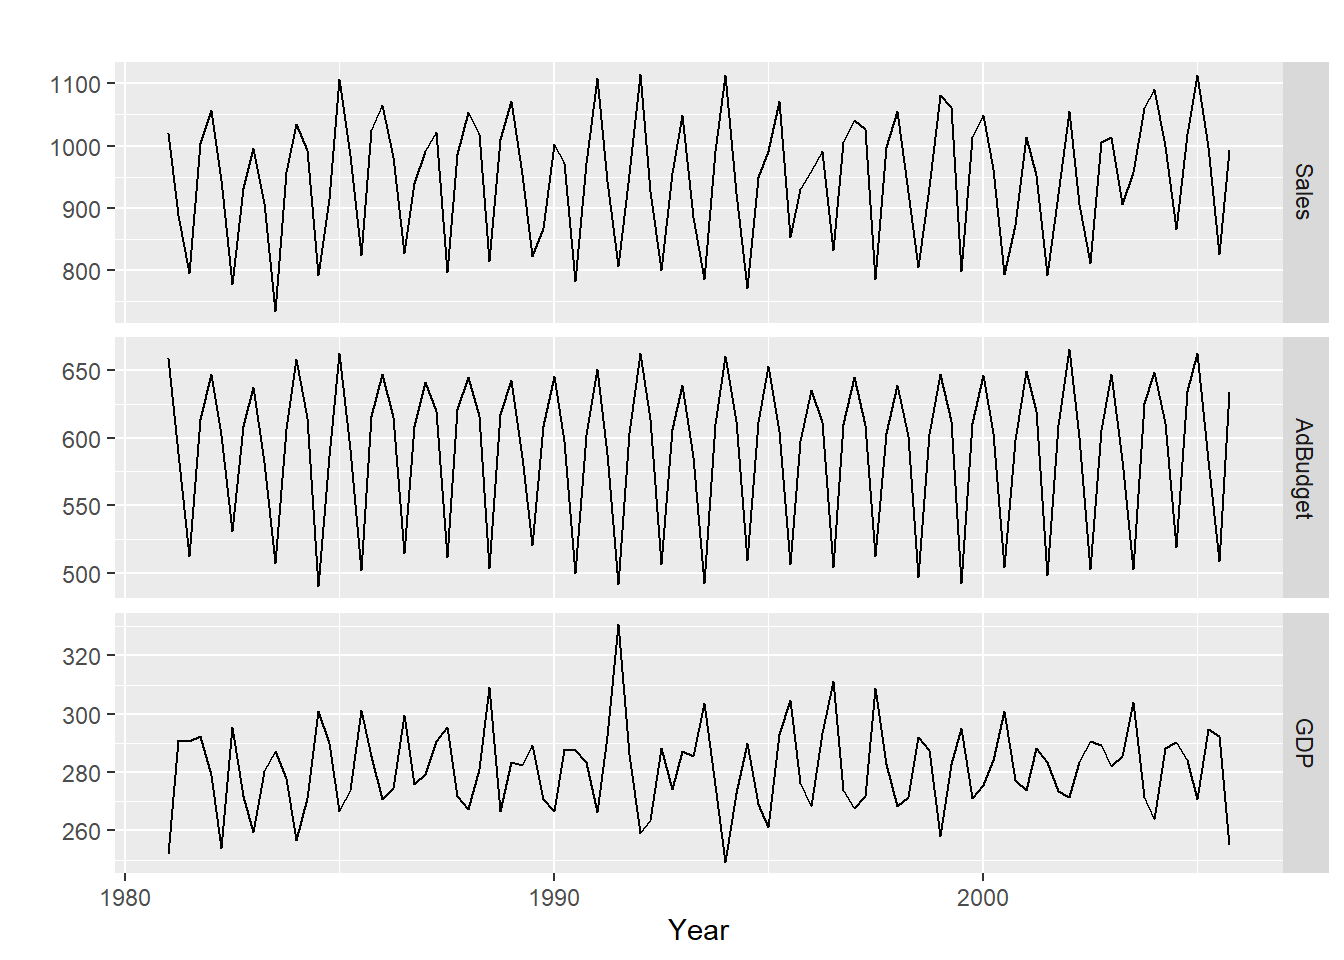
\includegraphics{thesis_files/figure-latex/deaths-1.pdf}
\caption{\label{fig:deaths}Quarterly sales, advertising and GDP data.}
\end{figure}

\hypertarget{results-from-analyses}{%
\section{Results from analyses}\label{results-from-analyses}}

We can fit a dynamic regression model to the sales data.

If \(y_t\) denotes the sales in quarter \(t\), \(x_t\) denotes the corresponding advertising budget and \(z_t\) denotes the GDP, then the resulting model is:
\begin{equation}
  y_t - y_{t-4} = \beta (x_t-x_{t-4}) + \gamma (z_t-z_{t-4}) + \theta_1 \varepsilon_{t-1} + \Theta_1 \varepsilon_{t-4} + \varepsilon_t
\end{equation}
where
\(\beta = 2.28\),
\(\gamma = 0.97\),
\(\theta_1 = NA\),
and
\(\Theta_1 = -0.90\).

\hypertarget{tables}{%
\section{Tables}\label{tables}}

Let's assume future advertising spend and GDP are at the current levels. Then forecasts for the next year are given in Table \ref{tab:salesforecasts}.

\begin{table}[ht]
\begin{center}
\begin{tabular}{lrrrr}
\toprule
Point Forecast & Lo 80 & Hi 80 & Lo 95 & Hi 95 \\
\midrule
1000.2 &  947.7 & 1052.7 & 919.9 & 1080.5 \\
1013.1 &  959.3 & 1066.8 & 930.9 & 1095.3 \\
1076.7 & 1022.9 & 1130.6 & 994.4 & 1159.0 \\
1003.5 &  949.7 & 1057.4 & 921.2 & 1085.8 \\
\bottomrule
\end{tabular}
\caption{Forecasts for the next year assuming Advertising budget and GDP are unchanged.}
\label{tab:salesforecasts}
\end{center}
\end{table}

Again, notice the use of labels and references to automatically generate table numbers. In this case, we need to generate the label ourselves.

The \texttt{knitLatex} package is useful for generating tables from R output. Other packages can do similar things including the \texttt{kable} function in \texttt{knitr} which is somewhat simpler but you have less control over the result. If you use \texttt{knitLatex} to generate tables, don't forget to include \texttt{results="asis"} in the chunk settings.

\hypertarget{sec:expsmooth}{%
\chapter{Exponential Smoothing}\label{sec:expsmooth}}

\hypertarget{organizing-your-ideas}{%
\section{Organizing your ideas}\label{organizing-your-ideas}}

Imagine you are writing for your fellow Honours students. Topics that are well-known to them do not have to be included here. But things that they may not know about should be included. Resist the temptation to discuss everything you've read in the last year.

Do not organize your chapter around the papers you have read with one section per paper. Instead, you should organize your chapters around themes, and within each theme provide a story explaining the development of ideas. It is usually helpful to plan out a table of contents first with major section headings.

When you are discussing results from several papers or books, you will need to adopt a common notation to ensure your chapter makes sense. Do not use different notation for the same thing.

\hypertarget{citations}{%
\section{Citations}\label{citations}}

All citations should be done using markdown notation as shown below. This way, your bibliography will be compiled automatically and correctly.

Exponential smoothing was originally developed in the late 1950s \autocite{Brown59,Brown63,Holt57,Winters60}. Because of their computational simplicity and interpretability, they became widely used in practice.

Empirical studies by \textcite{MH79} and \textcite{Metal82} found little difference in forecast accuracy between exponential smoothing and ARIMA models. This made the family of exponential smoothing procedures an attractive proposition \autocite[see][]{CKOS01}.

The methods were less popular in academic circles until \textcite{OKS97} introduced a state space formulation of some of the methods, which was extended in \textcite{HKSG02} to cover the full range of exponential smoothing methods.

\hypertarget{external-scripts}{%
\section{External Scripts}\label{external-scripts}}

You can include scripts that are \href{https://bookdown.org/yihui/rmarkdown-cookbook/option-code.html}{not directly embedded}
into the Rmd format
by using \texttt{code=xfun::read\_utf8("path/scripts/script.R")} in the chunk options eg:
\texttt{\{r\ echo=TRUE,\ code=xfun::read\_utf8(\textquotesingle{}scripts/histnorm.R\textquotesingle{})\}}:

\begin{Shaded}
\begin{Highlighting}[]
\CommentTok{\# histnorm.R}
\CommentTok{\# Takes 1000s draws of a normal distribution and plots it\textquotesingle{}s histogram}

\CommentTok{\# draw samples}
\NormalTok{vec }\OtherTok{\textless{}{-}} \FunctionTok{rnorm}\NormalTok{(}\DecValTok{1000}\NormalTok{)}

\CommentTok{\# plot histogram}
\FunctionTok{hist}\NormalTok{(vec)}
\end{Highlighting}
\end{Shaded}

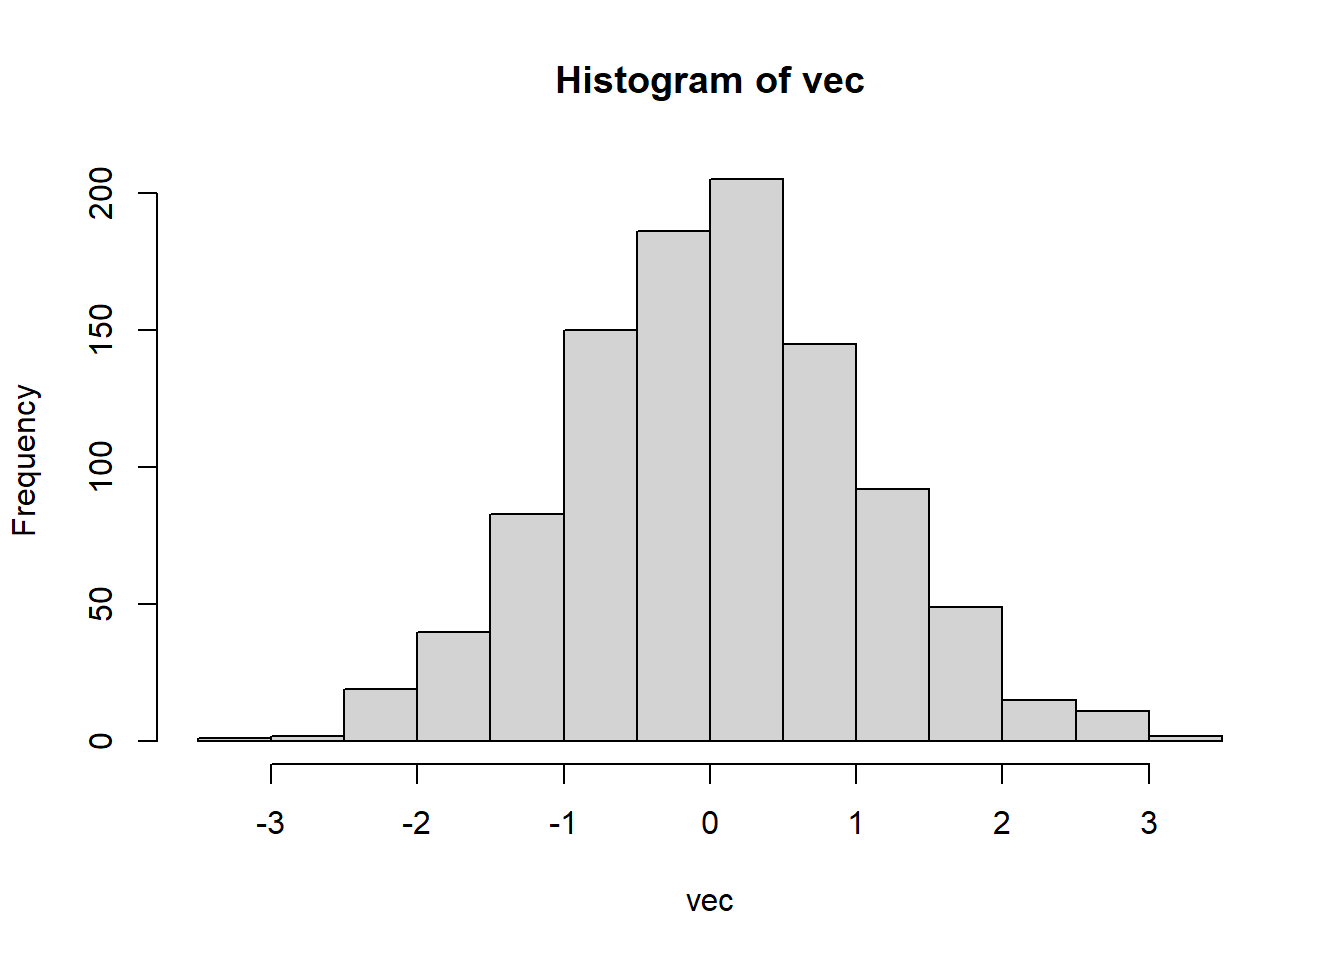
\includegraphics{thesis_files/figure-latex/unnamed-chunk-2-1.pdf}
or \href{https://bookdown.org/yihui/rmarkdown-cookbook/read-chunk.html}{by using labelled blocks in your script and using them as individual chunks}

\appendix

\hypertarget{additional-stuff}{%
\chapter{Additional stuff}\label{additional-stuff}}

You might put some computer output here, or maybe additional tables.

Note that line 5 must appear before your first appendix. But other appendices can just start like any other chapter.





%%%%%%%%%%%%%%%%%%%%%%%%%%%%%%%%%%%%%%%%%%%%%%%%%%%%%%%%%%%%%%%%%%%%%%%%%%

\clearpage


\printbibliography[title=References, heading=bibintoc]





\end{document}




